\clearpage
\subsection{Function Call} % (fold)
\label{sub:function_call}

A Function Call is used to execute a \nameref{sub:function}, and to read the value that is returned. This is similar to a \nameref{sub:procedure call}, but unlike a Procedure Call it must be done as part of an Expression.

\begin{figure}[h]
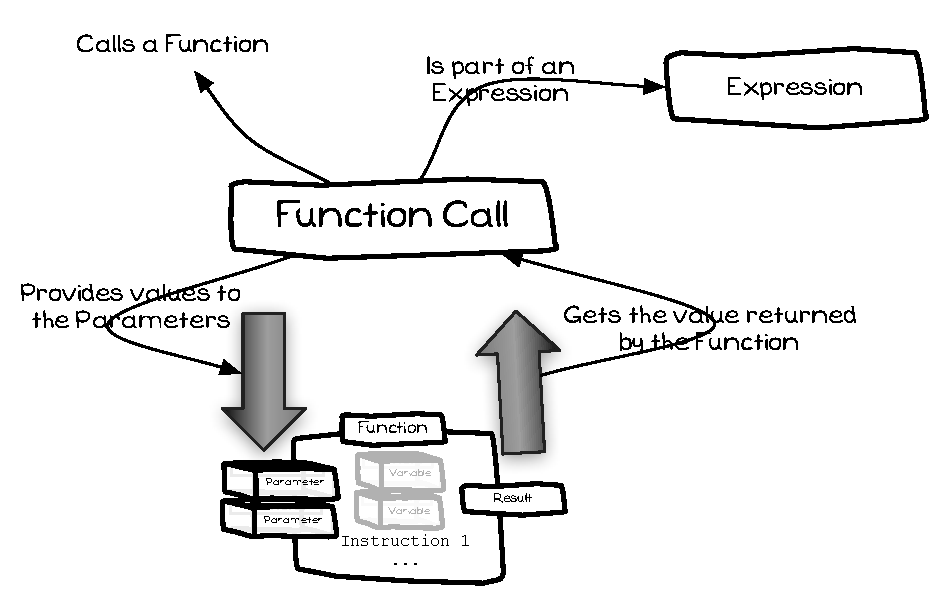
\includegraphics[width=\textwidth]{topics/storing-using-data/diagrams/FunctionCall} 
 \caption{A Function Call is part of an Expression where the value is calculated}
 \label{fig:storing-using-data-function-call}
\end{figure}

\mynote{
\begin{itemize}
  \item A Function Call is an \textbf{action}, but one that is performed as part of an Expression.
  \item Function calls can appear in \emph{any} expression. For example, you can use a Function Call to calculate the value in an \nameref{sub:assignment_statement}. You can use a Function Call to calculate the argument values for a Procedure Call.
\end{itemize}
}


% subsection function_call (end)